\documentclass[11pt]{article}
% =====================================================================
% arXiv-ready preprint. Compiles on Overleaf (pdfLaTeX) with no extra files.
% To adapt for MDPI Forecasting: paste the body into their official template.
% =====================================================================
\usepackage[utf8]{inputenc}
\usepackage[T1]{fontenc}
\usepackage{lmodern}
\usepackage[margin=1in]{geometry}
\usepackage{booktabs}
\usepackage{graphicx}
\usepackage{amsmath}
\usepackage{authblk}
\usepackage{hyperref}
\hypersetup{colorlinks=true, linkcolor=blue, citecolor=blue, urlcolor=blue}
\usepackage{microtype}
\usepackage{siunitx}

\title{\textbf{A Lightweight Temporal Fusion Transformer Matches\\
Billion-Scale Zero-Shot Foundation Models for Demand\\
Forecasting at a Fraction of the Cost}}

\author[1]{Adel Elsayed Mahmoud}
\affil[1]{Corresponding author: \texttt{adelelsayed1991@gmail.com}}
\date{\today}

\begin{document}
\maketitle

\begin{abstract}
\noindent
Time-series foundation models (TSFMs) such as Chronos, TimesFM, Moirai and TabPFN-TS
promise accurate, zero-shot forecasting without task-specific training, but they are
large ($10^8$--$10^9$ parameters), are often consumed through paid cloud APIs, and may
require sensitive data to leave an organisation's premises. We ask a practical question
for resource-constrained and privacy-sensitive deployments---particularly in healthcare
and pharmacy supply chains---\emph{whether a small, purpose-trained model can match these
foundation models.} We train a compact Temporal Fusion Transformer (TFT;
0.19--0.63 million parameters) and benchmark it head-to-head against four state-of-the-art
zero-shot TSFMs and a seasonal-naive baseline on two real demand datasets: NHS England
prescribing volumes (region $\times$ therapeutic-chapter, monthly) and the M5 retail
competition (item $\times$ store, weekly). Using identical evaluation windows, a clustered
(block) bootstrap over series, and a Diebold--Mariano test---repeated across three random
seeds---we find \textbf{no statistically significant difference between the lightweight TFT
and any foundation model on either dataset} (the paired confidence intervals on the WAPE
gap straddle zero in all cases). On M5 the TFT additionally and reproducibly outperforms the
seasonal-naive baseline; on the heavily aggregated NHS series no learned model---small or
large---beats seasonal-naive. We interpret ``no significant difference'' as failure to
detect a gap rather than proven equivalence (a formal equivalence test at a 10\%-of-naive
margin is not satisfied at our sample sizes). The TFT reaches this foundation-model-level
accuracy with a model 2--3 orders of magnitude smaller; for the NHS task it both trains and
serves on a commodity CPU with no data leaving the premises. For these demand series, a
small trained model is a competitive, far cheaper, and privacy-preserving alternative to
large zero-shot foundation models. We release all code, forecasts and analysis scripts for
full reproducibility.

\medskip
\noindent\textbf{Keywords:} demand forecasting; Temporal Fusion Transformer; time-series
foundation models; zero-shot forecasting; healthcare analytics; model efficiency;
reproducibility.
\end{abstract}

\section{Introduction}
Accurate short-horizon demand forecasting underpins inventory planning, budgeting and
capacity management. In healthcare and pharmacy supply chains specifically, forecasting
prescription and product demand affects medicine availability, waste, and cost control, and
is subject to two practical constraints that the recent literature rarely foregrounds:
\textbf{(i) data governance}---clinical and prescribing data frequently cannot be
transmitted to external cloud services; and \textbf{(ii) limited infrastructure}---many
providers operate modest on-premises hardware without dedicated GPUs.

The dominant recent trend in time-series machine learning is the \emph{foundation model}: a
large neural network pre-trained on enormous and diverse corpora that forecasts new series
\textbf{zero-shot}, i.e.\ with no task-specific training. Chronos~\cite{chronos},
TimesFM~\cite{timesfm}, Moirai~\cite{moirai} and TabPFN-TS~\cite{tabpfnts} exemplify this
paradigm. Their appeal is obvious---no training, strong out-of-the-box accuracy---but they
carry hidden costs for the constrained settings above: parameter counts in the hundreds of
millions, GPU or paid-API inference, and (for hosted variants) the need to send data
off-site.

This motivates the question we study: \emph{For real, operationally relevant demand series,
can a small, purpose-trained model---light enough to train once and serve on a CPU,
on-premises---match the accuracy of large zero-shot foundation models?} Our contributions
are:
\begin{enumerate}
\item \textbf{A fair, reproducible benchmark protocol} comparing a compact Temporal Fusion
Transformer against four TSFMs and a seasonal-naive baseline on \emph{identical} forecast
windows, in native demand units, with proper statistical testing (clustered bootstrap +
Diebold--Mariano) repeated over three seeds.
\item \textbf{Evidence on two contrasting real datasets}---NHS-EPD prescribing (monthly,
aggregated) and M5 retail (weekly, granular, covariate-rich)---showing the lightweight TFT
is statistically indistinguishable from every foundation model (no significant WAPE gap in
any of the four pairwise comparisons, on either dataset), while reproducibly beating the
seasonal-naive baseline on M5.
\item \textbf{A cost/efficiency analysis} quantifying the deployment gap: a 0.19--0.63\,M
parameter model, trainable in minutes-to-hours and served on CPU, versus $10^8$--$10^9$
parameter cloud/GPU models.
\item \textbf{Full artifact release} (code, per-seed forecasts, analysis scripts) enabling
exact reproduction of every reported number.
\end{enumerate}
We deliberately do \textbf{not} claim the TFT is the most accurate forecaster. Our claim is
the more useful one for practitioners: \emph{parity at a fraction of the cost and with
stronger data-governance properties.}

\section{Related Work}
\textbf{Temporal Fusion Transformer.} The TFT~\cite{tft} is an attention-based architecture
purpose-built for multi-horizon forecasting with heterogeneous inputs: static covariates,
known-future inputs (e.g.\ calendar, prices) and observed past inputs. Its variable-selection
networks and gated residual components provide both accuracy and interpretability. We use a
modernised TFT that combines the original TFT skeleton with components from contemporary
transformer practice: the Transformer self-attention block~\cite{transformer},
RMSNorm~\cite{rmsnorm}, rotary position embeddings (RoPE)~\cite{rope}, grouped-query
attention~\cite{gqa}, gated feed-forward layers (GLU variants)~\cite{glu}, and
FlashAttention~\cite{flash} for efficient exact attention, with a multi-quantile output head.

\textbf{Time-series foundation models.} Chronos tokenises values and applies a language-model
backbone; TimesFM is a patched decoder pre-trained on large real/synthetic corpora; Moirai is
a masked-encoder universal forecaster; TabPFN-TS adapts tabular in-context learning to time
series. All forecast zero-shot. Independent benchmarks report strong but not uniformly
dominant performance, and note that classical and lightweight baselines remain competitive on
many series---consistent with our findings.

\textbf{Efficiency and ``are foundation models worth it?''} A growing line of work questions
whether large pre-trained forecasters justify their cost relative to simple or small models.
We contribute a controlled, statistically tested, two-domain data point to this debate, with
an explicit healthcare-deployment lens.

\section{Data}
\subsection{NHS England Prescribing Dataset (EPD)}
The NHS Business Services Authority publishes monthly prescribing volumes. We construct series
at the \textbf{Regional Office $\times$ BNF chapter} level (the higher-level therapeutic
grouping recommended by the EPD release guidance when not using SNOMED-level detail), giving
\textbf{144 series over 65 months} (Nov 2020--Mar 2026). The target is monthly \textbf{items}
dispensed. Features: static categoricals (region, BNF chapter) and per-series scale
statistics; known-future calendar (month-of-year, sin/cos, trend); observed past (log-demand
history plus per-item cost/quantity proxies). The split is temporal: the final 12 months are
test, the preceding 6 are validation, the rest train. Encoder length $L=12$ months, horizon
$H=6$ months.

\subsection{M5 (Walmart) retail competition}
The M5 dataset~\cite{m5} contains daily unit sales of 30{,}490 item $\times$ store series
across 10 US stores. Daily item-level demand is highly intermittent (zero-inflated), which
suppresses learnable signal; we therefore \textbf{aggregate to weekly} resolution (summing
7-day buckets), yielding 278 weekly steps. We retain all sufficiently active series (28{,}175).
The target is weekly units. Features map cleanly to the three TFT channels: static
(department, category, store, state, plus per-series scale); \textbf{known-future}
(week-of-year sin/cos, trend, month, event type, \emph{and sell price}---set in advance by the
retailer); observed past (log-demand history, SNAP fraction). Encoder length $L=24$ weeks,
horizon $H=6$ weeks; the final 8 weeks are test, the preceding 8 validation.

The two datasets are deliberately contrasting: NHS-EPD is \textbf{few, smooth, heavily
aggregated} series; M5-weekly is \textbf{many, noisier, covariate-rich} series. Together they
probe whether the parity result is regime-dependent.

\section{Methods}
\subsection{Models}
\textbf{ModernTFT (ours).} A multi-quantile TFT (quantiles 0.1/0.25/0.5/0.75/0.9).
Configurations: NHS-EPD $d_{\text{model}}=64$ ($\approx$0.63\,M parameters); M5
$d_{\text{model}}=64$ with the M5 feature set ($\approx$0.19\,M parameters). Trained with
AdamW~\cite{adamw}, a cosine learning-rate schedule with linear warm-up and warm
restarts~\cite{sgdr}, a pinball (quantile) loss plus a small non-crossing penalty, and early
stopping on validation pinball loss.

\textbf{Foundation-model baselines (zero-shot).} Chronos-Bolt (base), TimesFM-2.5 (200\,M),
Moirai-1.1-R (large), TabPFN-TS (cloud client). Each receives the \emph{same} context window
the TFT saw and forecasts the same $H$ steps; quantiles are read or interpolated from each
model's native output.

\textbf{Seasonal-naive.} Repeats the value from one season ago; quantiles from in-sample
seasonal residuals. The standard sanity-check baseline.

\subsection{Fair-comparison protocol}
All models are scored on \textbf{identical (series, forecast-origin) windows}, in native
demand units (forecasts produced in log space are inverted via \texttt{expm1}). For M5,
evaluation is restricted to a stratified, seeded sample of 3{,}000 windows (the same windows
for every model) to keep cloud/GPU baselines tractable; NHS-EPD uses all 1{,}721 test windows.
Quantile predictions are clipped to be non-negative and sorted to enforce monotonicity for
every model alike.

\subsection{Metrics}
\textbf{WAPE} (weighted absolute percentage error, $\sum|e|/\sum|y|$)---volume-weighted point
accuracy; our headline metric. \textbf{MASE}~\cite{mase}---MAE relative to the in-sample
seasonal-naive MAE; $<1$ beats the naive scale. \textbf{RMSE}, \textbf{MAE}, \textbf{bias}.
\textbf{Pinball (quantile) loss}---the proper scoring rule and the model's training objective.
\textbf{Coverage} (empirical fraction inside the 80\% p10--p90 interval; nominal 0.80) and the
50\% p25--p75 interval---calibration.

\subsection{Statistical testing}
A single WAPE number can mislead because forecast rows are \textbf{not independent} (each
series contributes overlapping rolling windows $\times$ horizon steps); the effective sample
size is closer to the number of \emph{series}. We use two complementary tests on the
per-window error differential between the TFT and each rival:
(1)~a \textbf{cluster (block) bootstrap over series}~\cite{kunsch} (2{,}000 resamples):
resample whole series with replacement, recompute the WAPE gap each draw, report the 95\%
confidence interval (an interval excluding 0 is significant; straddling 0 is a tie);
(2)~a \textbf{Diebold--Mariano test}~\cite{dm} on the absolute-error differential with a
\textbf{series-clustered} standard error. We run the entire pipeline for \textbf{three random
seeds (42, 43, 44)} and report mean $\pm$ standard deviation, plus a robustness verdict
requiring agreement across all three seeds.

\section{Results}
All numbers below are regenerated by the released \texttt{analysis.py} from the per-seed
forecast files.

\subsection{NHS-EPD (monthly, 144 series, 1{,}721 test windows)}
\begin{table}[h]
\centering
\caption{NHS-EPD point and probabilistic accuracy. ModernTFT shown as mean $\pm$ std over
3 seeds; foundation models are zero-shot (seed-independent). RMSE in items.}
\begin{tabular}{lrrrr}
\toprule
Model & WAPE & MASE & RMSE & Coverage (80\%) \\
\midrule
SeasonalNaive & \textbf{0.0359} & \textbf{0.664} & \textbf{58{,}438} & 0.919 \\
\textbf{ModernTFT (ours)} & $0.0431 \pm 0.0029$ & $0.797 \pm 0.053$ & $66{,}353 \pm 4{,}926$ & 0.759 \\
TabPFN  & 0.0432 & 0.797 & 76{,}255 & 0.684 \\
TimesFM & 0.0440 & 0.813 & 78{,}891 & 0.803 \\
Moirai  & 0.0511 & 0.944 & 98{,}710 & 0.868 \\
Chronos & 0.0514 & 0.950 & 111{,}588 & 0.928 \\
\bottomrule
\end{tabular}
\end{table}

\noindent\textbf{Significance (across all 3 seeds).} Against the four foundation models the
TFT shows \textbf{no significant difference} in any case (bootstrap CIs straddle 0; per-seed
verdicts mix tie and TFT-better, never unanimous). The seasonal-naive baseline
\emph{significantly beats} the TFT in all three seeds---on these heavily aggregated, strongly
seasonal series, ``repeat last year'' is exceptionally hard to beat, and the foundation
models do not beat it either. Among the \emph{learned} models the TFT has the lowest RMSE,
though seasonal-naive's is lower still.

\subsection{M5 (weekly, 3{,}000 evaluation windows)}
\begin{table}[h]
\centering
\caption{M5 point and probabilistic accuracy. ModernTFT mean $\pm$ std over 3 seeds.}
\begin{tabular}{lrrrr}
\toprule
Model & WAPE & MASE & RMSE & Coverage (80\%) \\
\midrule
TimesFM & \textbf{0.4102} & \textbf{1.045} & 13{,}326 & 0.667 \\
Chronos & 0.4167 & 1.061 & 13{,}120 & 0.703 \\
\textbf{ModernTFT (ours)} & $0.4170 \pm 0.0093$ & $1.062 \pm 0.024$ & $14{,}156 \pm 433$ & \textbf{0.805} \\
TabPFN  & 0.4267 & 1.087 & 13{,}377 & 0.655 \\
Moirai  & 0.4399 & 1.121 & 14{,}497 & 0.660 \\
SeasonalNaive & 0.4773 & 1.216 & 14{,}616 & 0.771 \\
\bottomrule
\end{tabular}
\end{table}

\begin{table}[h]
\centering
\caption{M5 significance: WAPE gap (rival $-$ TFT) and verdict across 3 seeds.}
\begin{tabular}{lrl}
\toprule
Rival & WAPE gap (rival $-$ TFT) & Verdict across 3 seeds \\
\midrule
SeasonalNaive & $+0.054 \ldots +0.071$ & \textbf{TFT significantly better (all 3)} \\
Moirai  & $+0.016 \ldots +0.034$ & Tie (TFT better in 1/3) \\
TabPFN  & $+0.003 \ldots +0.020$ & Tie (TFT better in 1/3) \\
Chronos & $-0.007 \ldots +0.010$ & Tie (all 3) \\
TimesFM & $-0.014 \ldots +0.004$ & Tie (TimesFM better in 1/3) \\
\bottomrule
\end{tabular}
\end{table}

\noindent The TFT is \textbf{statistically tied with all four foundation models}, sits
mid-pack on WAPE, and is the \textbf{best-calibrated} model (80\% coverage 0.805,
essentially nominal, versus 0.66--0.70 for the strongest TSFMs, which are over-confident). It
significantly and reproducibly beats the seasonal-naive baseline.

\subsection{Cost and deployment (the central finding)}
\begin{table}[h]
\centering
\caption{Model size and deployment profile.}
\begin{tabular}{lllll}
\toprule
Model & Parameters & Training & Inference & Data off-site? \\
\midrule
\textbf{ModernTFT (ours)} & \textbf{0.19--0.63\,M} & once: 9--14 min (NHS, CPU) / & CPU (NHS) & \textbf{No} \\
 & & 8.8--10.6\,h (M5, 1 GPU) & & \\
Chronos-Bolt base & $\approx$200\,M & none (zero-shot) & GPU & host-dependent \\
TimesFM-2.5 & 200\,M & none & GPU & host-dependent \\
Moirai-1.1-R large & $\approx$311\,M & none & GPU & host-dependent \\
TabPFN-TS & $\approx$11\,M (cloud client) & none & \textbf{cloud API} & \textbf{Yes (hosted)} \\
\bottomrule
\end{tabular}
\end{table}

\noindent The TFT is \textbf{2--3 orders of magnitude smaller} than the neural TSFMs. At this
size CPU inference is feasible and was used end-to-end for NHS-EPD; for the larger M5 corpus we
trained on a single GPU. Crucially, the model and data remain on-premises for both tasks,
unlike a hosted-API baseline such as TabPFN-TS.

\begin{figure}[h]
\centering
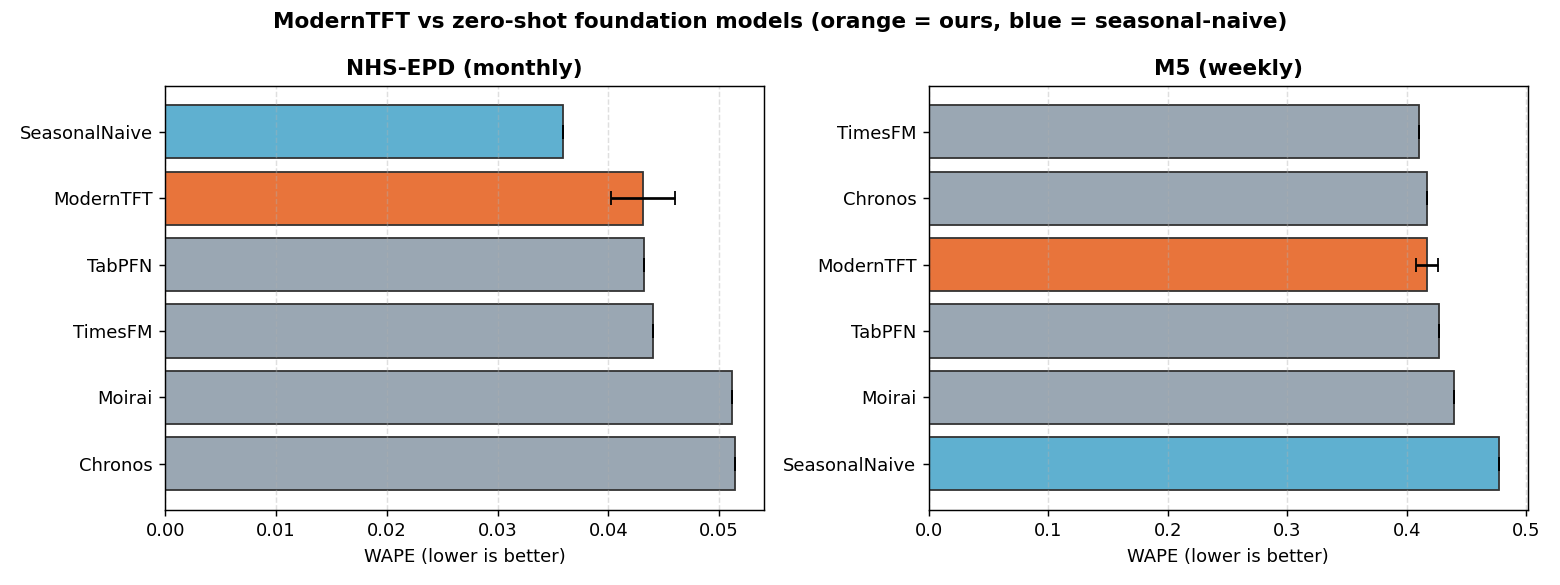
\includegraphics[width=\textwidth]{figures/fig1_wape.png}
\caption{WAPE comparison (orange = our TFT, with $\pm$std error bar across 3 seeds; blue =
seasonal-naive). The TFT sits among the foundation models on both datasets.}
\end{figure}
\begin{figure}[h]
\centering
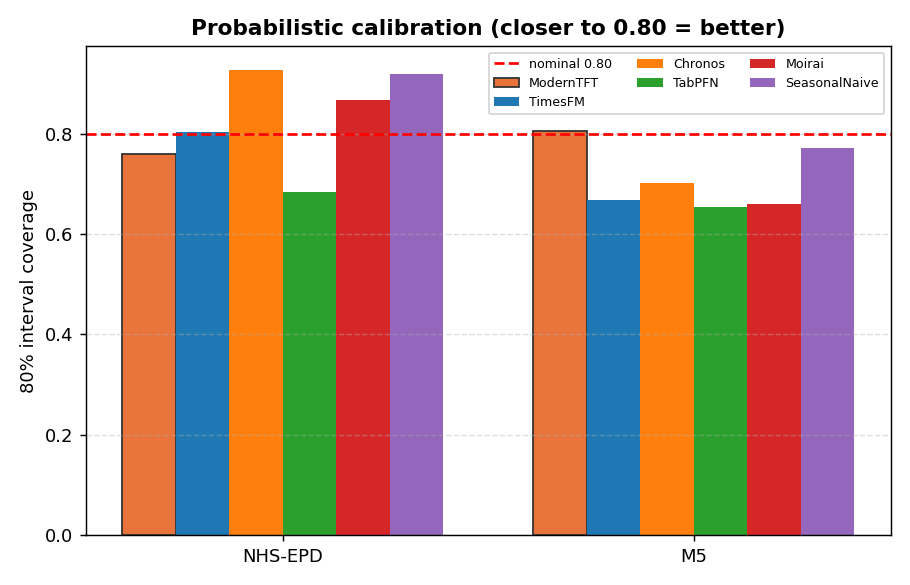
\includegraphics[width=0.75\textwidth]{figures/fig2_calibration.png}
\caption{80\% prediction-interval coverage (nominal 0.80, dashed). The TFT is well-calibrated
on M5; the strongest TSFMs are over-confident.}
\end{figure}
\begin{figure}[h]
\centering
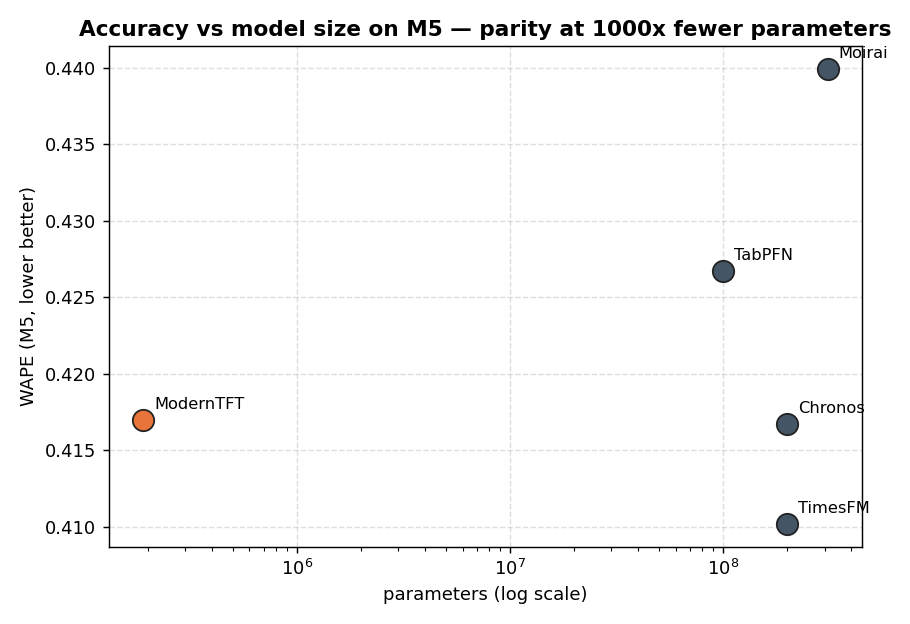
\includegraphics[width=0.75\textwidth]{figures/fig3_cost_accuracy.png}
\caption{M5 accuracy vs.\ model size (log scale): comparable WAPE at $\sim$1000$\times$ fewer
parameters.}
\end{figure}

\section{Discussion}
\textbf{The headline.} Across two contrasting real demand datasets, a sub-million-parameter,
CPU-servable TFT is \textbf{statistically indistinguishable from four billion-scale zero-shot
foundation models}, and is better calibrated than the strongest of them on M5. Neither the
small model nor the large models beat a seasonal-naive baseline on the heavily aggregated NHS
series---a useful caution that, when demand is smooth and dominated by annual seasonality,
sophisticated models add little over a strong classical baseline.

\textbf{Why this matters for healthcare/pharmacy.} The constraints that make TSFMs awkward in
clinical settings---cloud dependency, GPU requirements, data egress---are exactly where the
lightweight TFT is advantageous. A model that trains in minutes on CPU and serves on existing
on-premises hardware, with accuracy matching the state of the art, is operationally preferable
for prescribing- and product-demand forecasting under data-governance constraints.

\textbf{Regime dependence.} The two datasets bracket the practical spectrum. On
few/smooth/aggregated series (NHS), all learned models converge to roughly the seasonal-naive
frontier. On many/granular/covariate-rich series (M5-weekly), the trained TFT exploits
known-future covariates (notably price and events) and pulls clear of the naive baseline while
matching the TSFMs. In both regimes, \emph{training a small specialist is sufficient to reach
the foundation-model frontier.}

\textbf{Calibration.} Beyond point accuracy, the TFT's prediction intervals were close to
nominal coverage on M5 (0.805 vs.\ 0.80), whereas TimesFM and Chronos were over-confident
(0.66--0.70). For inventory decisions driven by quantiles (safety stock), calibration matters
as much as the median.

\section{Limitations}
\begin{itemize}
\item \textbf{``No significant difference'' is not proven equivalence.} Our central claim rests
on \emph{failing to reject} a difference. A formal equivalence (TOST-style) test requiring the
95\% bootstrap CI of the WAPE gap to fall within $\pm$10\% of the seasonal-naive WAPE is
\textbf{not} satisfied at our sample sizes. We claim indistinguishability at the tested power,
not equivalence.
\item \textbf{Only three seeds.} Per-seed verdicts occasionally flip (e.g.\ TimesFM beats the
TFT in 1/3 M5 seeds), which is why we report the full per-seed table. A larger seed budget
would tighten estimates.
\item \textbf{Two datasets, one domain family (demand).}
\item \textbf{M5 uses a 3{,}000-window stratified sample} of the busiest series, single
sampling seed; extreme-tail intermittent series are under-represented.
\item \textbf{MASE $>1$ on M5} reflects the 6-week horizon and weekly retail intermittency; it
is not unique to our model (all models exceed 1 there).
\item \textbf{Foundation models are evaluated zero-shot}; fine-tuning was out of scope.
\item \textbf{Single context configuration per dataset.}
\item \textbf{Hyperparameter sensitivity.} Training was sensitive to learning rate
(a 10$\times$ increase caused divergence); we report a stable configuration.
\end{itemize}

\section{Conclusion}
For demand forecasting under real-world constraints, a lightweight, purpose-trained Temporal
Fusion Transformer matches the accuracy of large zero-shot time-series foundation
models---statistically tied on two contrasting datasets, better calibrated on the granular
one, and significantly better than a seasonal-naive baseline where any model can be. It does
so at 2--3 orders of magnitude fewer parameters, with CPU inference and full on-premises data
control. Where infrastructure, budget, or data governance are binding---as they routinely are
in healthcare and pharmacy---a small trained model is a credible, cheaper, and safer
alternative to billion-scale foundation models. We release all code and forecasts to support
replication and extension.

\section*{Declaration on the use of AI tools}
The authors used an AI assistant (Anthropic Claude) to support code development, analysis
scripting, figure generation, and manuscript drafting. All quantitative results were produced
by the authors' own code (\texttt{analysis.py} and the released pipelines) and were verified
by the authors. The authors take full responsibility for the content of this article.

\section*{Data availability}
NHS English Prescribing Dataset (EPD, with SNOMED code), NHS Business Services Authority Open
Data Portal, \url{https://opendata.nhsbsa.net/dataset/english-prescribing-dataset-epd-with-snomed-code}
(accessed June 2026), Open Government Licence. M5 Forecasting -- Accuracy, Kaggle,
\url{https://www.kaggle.com/competitions/m5-forecasting-accuracy}. Code, per-seed forecasts and
analysis scripts are archived on Zenodo, DOI: \href{https://doi.org/10.5281/zenodo.21189124}{10.5281/zenodo.21189124}.
Preprint DOI: \href{https://doi.org/10.5281/zenodo.21189175}{10.5281/zenodo.21189175}.

\begin{thebibliography}{99}
\bibitem{chronos} A.~F.~Ansari et al. Chronos: Learning the Language of Time Series.
\emph{TMLR}, 2024. arXiv:2403.07815.
\bibitem{timesfm} A.~Das, W.~Kong, R.~Sen, Y.~Zhou. A decoder-only foundation model for
time-series forecasting (TimesFM). \emph{ICML}, 2024. arXiv:2310.10688.
\bibitem{moirai} G.~Woo, C.~Liu, A.~Kumar, C.~Xiong, S.~Savarese, D.~Sahoo. Unified Training
of Universal Time Series Forecasting Transformers (Moirai). \emph{ICML}, 2024. arXiv:2402.02592.
\bibitem{tabpfnts} S.~B.~Hoo, S.~M\"uller, D.~Salinas, F.~Hutter. From Tables to Time:
Extending TabPFN-v2 to Time Series Forecasting (TabPFN-TS). 2025. arXiv:2501.02945.
\bibitem{tft} B.~Lim, S.~\"O.~Ar\i k, N.~Loeff, T.~Pfister. Temporal Fusion Transformers for
interpretable multi-horizon time series forecasting. \emph{Int. J. Forecasting},
37(4):1748--1764, 2021.
\bibitem{m5} S.~Makridakis, E.~Spiliotis, V.~Assimakopoulos. The M5 competition: Background,
organization, and implementation. \emph{Int. J. Forecasting}, 38(4):1325--1336, 2022.
\bibitem{transformer} A.~Vaswani et al. Attention Is All You Need. \emph{NeurIPS}, 2017.
\bibitem{rope} J.~Su, Y.~Lu, S.~Pan, A.~Murtadha, B.~Wen, Y.~Liu. RoFormer: Enhanced
Transformer with Rotary Position Embedding. 2021. arXiv:2104.09864.
\bibitem{rmsnorm} B.~Zhang, R.~Sennrich. Root Mean Square Layer Normalization. \emph{NeurIPS},
2019. arXiv:1910.07467.
\bibitem{gqa} J.~Ainslie, J.~Lee-Thorp, M.~de~Jong, Y.~Zemlyanskiy, F.~Lebr\'on, S.~Sanghai.
GQA: Training Generalized Multi-Query Transformer Models from Multi-Head Checkpoints.
\emph{EMNLP}, 2023. arXiv:2305.13245.
\bibitem{glu} N.~Shazeer. GLU Variants Improve Transformer. 2020. arXiv:2002.05202.
\bibitem{adamw} I.~Loshchilov, F.~Hutter. Decoupled Weight Decay Regularization (AdamW).
\emph{ICLR}, 2019. arXiv:1711.05101.
\bibitem{sgdr} I.~Loshchilov, F.~Hutter. SGDR: Stochastic Gradient Descent with Warm Restarts.
\emph{ICLR}, 2017. arXiv:1608.03983.
\bibitem{flash} T.~Dao, D.~Y.~Fu, S.~Ermon, A.~Rudra, C.~R\'e. FlashAttention: Fast and
Memory-Efficient Exact Attention with IO-Awareness. \emph{NeurIPS}, 2022. arXiv:2205.14135.
\bibitem{dm} F.~X.~Diebold, R.~S.~Mariano. Comparing predictive accuracy. \emph{J. Business
\& Economic Statistics}, 13(3):253--263, 1995.
\bibitem{mase} R.~J.~Hyndman, A.~B.~Koehler. Another look at measures of forecast accuracy.
\emph{Int. J. Forecasting}, 22(4):679--688, 2006.
\bibitem{kunsch} H.~R.~K\"unsch. The jackknife and the bootstrap for general stationary
observations. \emph{Annals of Statistics}, 17(3):1217--1241, 1989.
\end{thebibliography}

\end{document}
